%%%% debut macro %%%%
\def\keepspace{\ifnum\catcode`\ =10
  \let\next\keepspacebis \else \let\next\relax \fi
  \next}
\def \keepspacebis{\obeyspaces
  \afterassignment\keepspaceaux\let\next= }
{\obeyspaces%
\gdef\keepspaceaux{%
\ifx \next\space\let\next\ignorespaces\fi%
\catcode`\  =10\relax\next}}
%%%%
%%%% fin macro %%%%
%\newcommand{\noteperso}[1]{\begin{center}
%\fbox{\begin{minipage}{.8\textwidth}#1\end{minipage}}\end{center}}


\addto\captionsfrench{\renewcommand{\tablename}{\textsc{Tableau}}}
%\renewcommand\listfigurename{Liste des figures}
\renewcommand{\thefootnote}{\fnsymbol{footnote}}
\newcommand{\ie}{\emph{i.e.}\xspace}
\newcommand{\cad}{c'est-à-dire\xspace}
\newcommand{\via}{\emph{via}\xspace}
\newcommand{\apriori}{\emph{a priori}\xspace}
\newcommand{\aposteriori}{\emph{a posteriori}\xspace}
\newcommand{\afortiori}{\emph{a fortiori}\xspace}
\newcommand{\adhoc}{\emph{ad hoc}\xspace}
\newcommand{\resp}{{\em resp.}\xspace}
\newcommand{\cf}{\emph{cf.}\xspace}
\newcommand{\na}{\mbox{n/a}\xspace}
\newcommand{\eg}{\emph{e.g.}\xspace}
\newcommand{\superscript}[1]{\ensuremath{^{\textrm{#1}}}}
\newcommand{\subscript}[1]{\ensuremath{_{\textrm{#1}}}}
\newcommand{\prev}{{\em précédente}\xspace}
\newcommand{\suiv}{{\em suivante}\xspace}
\newcommand{\comnet}{{\em Complex Networks}\xspace}
\DeclareUrlCommand\printtopic{\urlstyle{tt}}
\newcommand{\topic}[1]{\protect\printtopic{#1}\index{#1}\xspace}
\newcommand{\rfc}[1]{~\cite{rfc#1}\xspace}
\newcommand{\etal}{{\em et al.}\xspace}
\newcommand{\cat}[1]{#1\xspace}
\newcommand{\frames}{{\em frames}\xspace}
\newcommand{\ip}{{\sc IP}\xspace}
\newcommand{\mac}{{\sc MAC}\xspace}
\newcommand{\tcp}{{\sc TCP}\xspace}
\newcommand{\udp}{{\sc UDP}\xspace}
\newcommand{\bgp}{{\sc BGP}\xspace}
\newcommand{\ospf}{{\sc OSPF}\xspace}
\newcommand{\icmp}{{\sc ICMP}\xspace}
\newcommand{\mbone}{{\sc MBONE}\xspace}
\newcommand{\http}{{\sc HTTP}\xspace}
\newcommand{\https}{{\sc HTTPS}\xspace}
\newcommand{\tls}{{\sc TLS}\xspace}
\newcommand{\ssl}{{\sc SSL}\xspace}
\newcommand{\ttl}{{\sc TTL}\xspace}
\newcommand{\LL}{{\sc L2}\xspace}
\newcommand{\LLL}{{\sc L3}\xspace}
\newcommand{\LLLL}{{\sc L4}\xspace}
\newcommand{\icmptimeout}{{\sc ICMP}~{\sc Time Exceeded}\xspace}
\newcommand{\traceroute}{{\sc traceroute}\xspace}
\newcommand{\tracetree}{{\sc tracertree}\xspace}
\newcommand{\paristraceroute}{{\sc paris traceroute}\xspace}
\newcommand{\mrinfo}{{\sc mrinfo}\xspace}
\newcommand{\ping}{{\sc ping}\xspace}
\newcommand{\ssh}{{\sc ssh}\xspace}
\newcommand{\iffinder}{{\em iffinder}\xspace}
\newcommand{\udpping}{{\sc UDP Ping}\xspace}
\newcommand{\udpexplore}{{\sc UDP Explore}\xspace}
\newcommand{\AS}{{\em Autonomous System}\xspace}
\newcommand{\ASes}{{\em Autonomous Systems}\xspace}
\newcommand{\as}{{\em AS}\xspace}
\newcommand{\planetlab}{{\em Planetlab}\xspace}
\newcommand{\dimes}{{\em DIMES}\xspace}
\newcommand{\ripeatlas}{{\em RIPE Atlas}\xspace}
\newcommand{\switch}{{\em switch}\xspace}
\newcommand{\hop}{{\em hop}\xspace}
\newcommand{\cidr}{{\em CIDR}\xspace}
\newcommand{\iana}{{\em IANA}\xspace}

\newcommand{\reffig}[1]{{\bf Figure~\ref{fig:#1}}\xspace}
\newcommand{\reftable}[1]{{\bf Tableau~\ref{table:#1}\xspace}}
\newcommand{\refalg}[1]{{\bf Algorithme~\ref{alg:#1}}\xspace}
\newcommand{\refchap}[1]{{\bf Chapitre~\ref{chap:#1}}\xspace}
\newcommand{\refsec}[1]{{\bf Section~\ref{sec:#1}}\xspace}
\newcommand{\refsubsec}[1]{{\bf Section~\ref{subsec:#1}}\xspace}
\newcommand{\refsubsubsec}[1]{{\bf Section~\ref{subsubsec:#1}}\xspace}
\newcommand{\refdef}[1]{{\bf Définition~\ref{def:#1}}\xspace}
\newcommand{\refhyp}[1]{{\bf Hypothèse~\ref{hyp:#1}}\xspace}
\newcommand{\refprop}[1]{{\bf Proposition~\ref{prop:#1}}\xspace}
\newcommand{\refapp}[1]{{\bf Annexe~\ref{app:#1}}\xspace}

\makeatletter
\newcommand{\phfig}[3]{
\begin{figure}[!ht]
\centering
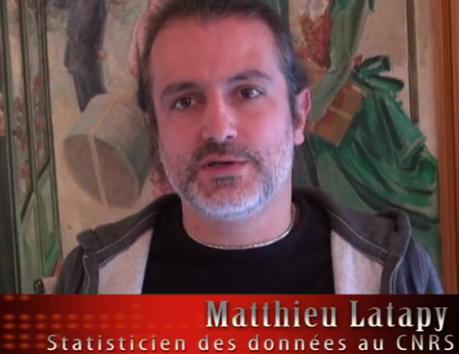
\includegraphics[width=\columnwidth]{images/mlatapy.png} \caption[#1]{#2}
\label{fig:#3} 
\end{figure}}
\makeatother

\makeatletter
\newcommand{\realfig}[4]{
\begin{figure}[!ht]
\centering
\includegraphics[width=\columnwidth]{images/#1} \caption[#2]{#3}
\label{fig:#4} 
\end{figure}}
\makeatother

\makeatletter
\newcommand{\realfigauto}[4]{
\begin{figure}[!htbp]
\centering
\makebox[\columnwidth]{\includegraphics[width=0.9\paperwidth]{images/#1}}
\caption[#2]{#3}
\label{fig:#4} 
\end{figure}}
\makeatother

\makeatletter
\newsavebox\myboxA
\newsavebox\myboxB
\newlength\mylenA

\newcommand{\pairs}[1]{#1 \times #1}
% \left(
% \begin{array}{c}
% #1\\
% 2\\
% \end{array}
% \right)
% }


\newcommand*\xoverline[2][0.75]{%
    \sbox{\myboxA}{$\m@th#2$}%
    \setbox\myboxB\null% Phantom box
    \ht\myboxB=\ht\myboxA%
    \dp\myboxB=\dp\myboxA%
    \wd\myboxB=#1\wd\myboxA% Scale phantom
    \sbox\myboxB{$\m@th\overline{\copy\myboxB}$}%  Overlined phantom
    \setlength\mylenA{\the\wd\myboxA}%   calc width diff
    \addtolength\mylenA{-\the\wd\myboxB}%
    \ifdim\wd\myboxB<\wd\myboxA%
       \rlap{\hskip 0.5\mylenA\usebox\myboxB}{\usebox\myboxA}%
    \else
        \hskip -0.5\mylenA\rlap{\usebox\myboxA}{\hskip 0.5\mylenA\usebox\myboxB}%
    \fi}
\makeatother

\newcommand{\ecite}{{\em \tt \small (citation manquante)}\xspace}
\newcommand{\tocite}[1]{{\em \tt \small [? #1]}\xspace}

\newcommand{\fixthis}{{\em \bf (FIXTHIS)}\xspace}

\newcommand{\attention}{{\textsc{\bf attention}}\xspace}

\newcommand{\IPSet}{\mathbb{I}}
\newcommand{\fonction}[5]{\begin{array}{lrcl}
#1: & #2 & \longrightarrow & #3 \\
    & #4 & \longmapsto & #5 \end{array}
}
\newcommand{\fonc}[3]{\begin{array}{llcl}
#1: & #2 & \longmapsto & #3 \end{array}
}

\usepackage{pgffor, ifthen}
\newcommand{\notes}[3][\empty]{%
  \noindent Notes\vspace{10pt}\\
  \foreach \n in {1,...,#2}{%
    \ifthenelse{\equal{#1}{\empty}}
      {\rule{#3}{0.5pt}\\}
      {\rule{#3}{0.5pt}\vspace{#1}\\}
    }
}

\makeatletter

\def\@newbackl@bel#1#2#3{%
 \@ifundefined{#1@#2}%
  {\global\@namedef{#1@#2}{#3}}
  {\cs@g@appendpair{#1@#2}{#3}}%
}
% #1 and #2 are each of the form {a}{b}, and the a and b groups are to be concatenated independently.
\def\cs@g@appendpair#1#2{{%
 \edef\first{\csname #1\endcsname}%
 \csxdef{#1}%
  {{\expandafter\@firstoftwo\first,\@firstoftwo#2}%
   {\expandafter\@secondoftwo\first,\@secondoftwo#2}}%
}}

%###
% Patching into the existing commands
\def\newbacklabel{\@newbackl@bel B}
\let\backlabel=\label
\patchcmd\backlabel{\newlabel}{\newbacklabel}{}{}
\let\backref=\ref
\patchcmd\backref{r@#1}{B@#1}{}{}
\let\pagebackref=\pageref
\patchcmd\pagebackref{r@#1}{B@#1}{}{}
\pretocmd\ref{\backlabel{#1}}{}{}

\makeatother

%###



\algrenewcommand{\algorithmiccomment}[1]{\# \textit{#1}}

\newcommand{\fcite}[1]{\todo[color=green!40]{#1}}
\newcommand{\conclu}[1]{\todo[color=red!40]{#1}}

\newcommand{\todoa}[1]{\todo[inline]{#1}}

\newcommand{\rem}[1]{\todo[nolist,color=yellow!40]{#1}\xspace}
\newcommand{\remi}[1]{\smallskip\todo[inline,nolist,color=yellow!40]{#1}\xspace\smallskip}
\newcommand{\res}[1]{\todo[nolist,color=blue!40]{#1}\xspace}
\newcommand{\arelire}{\todo[inline,nolist,color=blue!40]{\`A relire}\xspace}
\newcommand{\non}[1]{\todo[inline,nolist,color=red!40]{#1}}

\newcommand{\clem}[1]{\todo[inline,author=clemence,color=orange!40]{#1}}

%\newcommand{\bof}{\todo[nolist,color=red!40]{Bôf}\xspace}
\newcommand{\bof}[1]{\underline{#1}{\bf (bof)}\xspace}


\specialcomment{fauxtexte}{\begingroup\ttfamily}{\endgroup}
\specialcomment{atraduire}{\begingroup}{\endgroup}
\specialcomment{contenu}{\begingroup}{\endgroup}

\specialcomment{motivation}{\begingroup\begin{center}\begin{minipage}{.8\textwidth}\begin{mdframed}[roundcorner=10pt]Motivation : }{\end{mdframed}\end{minipage}\end{center}\endgroup}

\specialcomment{encadre}{\bigskip\begingroup\begin{center}\begin{minipage}{.8\textwidth}\begin{mdframed}[roundcorner=10pt]}{\end{mdframed}\end{minipage}\end{center}\endgroup\bigskip}

\specialcomment{noteperso}{\begingroup\begin{center}\begin{minipage}{.8\textwidth}Note perso : }{\end{minipage}\end{center}\endgroup}

\excludecomment{atraduire}
%\excludecomment{contenu}
\excludecomment{fauxtexte}
%\excludecomment{encadre}
%\excludecomment{contribution}
%\excludecomment{motivation}

%\newcommand{\listcontributionname}{Liste des contributions}
%\newlistof{contributions}{ctb}{\listcontributionname}
%\newcommand{\contribution}[1]{#1 $\clubsuit$%
%\refstepcounter{contributions}%
%\addcontentsline{ctb}{contributions}{#1}}

%\newcommand{\listconclusionname}{Liste des éléments de conclusion}
%\newlistof{conclusions}{ccl}{\listconclusionname}
%\newcommand{\conclusion}[1]{#1 $\spadesuit$%
%\refstepcounter{conclusions}%
%\addcontentsline{ccl}{conclusions}{#1}}

%\newcommand{\listperspectivename}{Liste des perspectives}
%\newlistof{perspectives}{psp}{\listperspectivename}
%\newcommand{\perspective}[1]{#1 $\P$%
%\refstepcounter{perspectives}%
%\addcontentsline{psp}{perspectives}{#1}}

\newcommand{\includegraphicsmaybe}[2][]{\IfFileExists{#2}{\includegraphics{#2}}{\fbox{#2 is missing}\\}}
%\newcommand{\includegraphicsmaybe}[1]{\IfFileExists{#1}{\includegraphics{#1}}{\makebox[0pt]{File #1 is missing}\includegraphics{dessin.pdf}}}
%\renewcommand{\includegraphics}[2][]{\fbox{#2}}
%\newcommand{\includegraphicsmaybe}{\includegraphics}
\renewcommand{\appendixtocname}{Annexes} 
\renewcommand{\appendixpagename}{Annexes} 
\newcommand{\blankpage}{
\newpage
\thispagestyle{empty}
\mbox{}
\newpage
}

\hyphenation{gau-ging}
\hyphenation{mum-my}
%
\hyphenation{re-cher-che}
\hyphenation{pro-bl\'e-ma-tique}
\hyphenation{\'evo-lu-tion}
\hyphenation{si-gni-fi-ca-ti-vement}
\hyphenation{finale-ment}
\hyphenation{con-tient}
\hyphenation{cour-bes}
\hyphenation{cha-que}
\hyphenation{princi-pa-le-ment}
\hyphenation{con-cep-tion}
\hyphenation{con-damnées}
\hyphenation{iden-ti-fiées}
\hyphenation{con-nectées}
\hyphenation{ens-emble}


